% This contents of this file will be inserted into the _Solutions version of the
% output tex document.  Here's an example:

% If assignment with subquestion (1.a) requires a written response, you will
% find the following flag within this document: <SCPD_SUBMISSION_TAG>_1a
% In this example, you would insert the LaTeX for your solution to (1.a) between
% the <SCPD_SUBMISSION_TAG>_1a flags.  If you also constrain your answer between the
% START_CODE_HERE and END_CODE_HERE flags, your LaTeX will be styled as a
% solution within the final document.

% Please do not use the '<SCPD_SUBMISSION_TAG>' character anywhere within your code.  As expected,
% that will confuse the regular expressions we use to identify your solution.
\def\assignmentnum{1 }
\def\assignmenttitle{XCS330 Problem Set \assignmentnum}

\documentclass{article}
\usepackage[top = 1.0in]{geometry}

\usepackage{graphicx}

\usepackage[utf8]{inputenc}
\usepackage{listings}
\usepackage[dvipsnames]{xcolor}
\usepackage{bm}
\usepackage{algorithm}
\usepackage{algpseudocode}
\usepackage{framed}
\usepackage{xspace}

\definecolor{codegreen}{rgb}{0,0.6,0}
\definecolor{codegray}{rgb}{0.5,0.5,0.5}
\definecolor{codepurple}{rgb}{0.58,0,0.82}
\definecolor{backcolour}{rgb}{0.95,0.95,0.92}

\lstdefinestyle{mystyle}{
    backgroundcolor=\color{backcolour},   
    commentstyle=\color{codegreen},
    keywordstyle=\color{magenta},
    stringstyle=\color{codepurple},
    basicstyle=\ttfamily\footnotesize,
    breakatwhitespace=false,         
    breaklines=true,                 
    captionpos=b,                    
    keepspaces=true,                 
    numbersep=5pt,                  
    showspaces=false,                
    showstringspaces=false,
    showtabs=false,                  
    tabsize=2
}

\lstset{style=mystyle}

\newcommand{\di}{{d}}
\newcommand{\nexp}{{n}}
\newcommand{\nf}{{p}}
\newcommand{\vcd}{{\textbf{D}}}
\newcommand{\Int}{\mathbb{Z}}
\newcommand\bb{\ensuremath{\mathbf{b}}}
\newcommand\bs{\ensuremath{\mathbf{s}}}
\newcommand\bp{\ensuremath{\mathbf{p}}}
\newcommand{\relu} { \operatorname{ReLU} }
\newcommand{\smx} { \operatorname{softmax} }
\newcommand\bx{\ensuremath{\mathbf{x}}}
\newcommand\bh{\ensuremath{\mathbf{h}}}
\newcommand\bc{\ensuremath{\mathbf{c}}}
\newcommand\bW{\ensuremath{\mathbf{W}}}
\newcommand\by{\ensuremath{\mathbf{y}}}
\newcommand\bo{\ensuremath{\mathbf{o}}}
\newcommand\be{\ensuremath{\mathbf{e}}}
\newcommand\ba{\ensuremath{\mathbf{a}}}
\newcommand\bu{\ensuremath{\mathbf{u}}}
\newcommand\bv{\ensuremath{\mathbf{v}}}
\newcommand\bP{\ensuremath{\mathbf{P}}}
\newcommand\bg{\ensuremath{\mathbf{g}}}
\newcommand\bX{\ensuremath{\mathbf{X}}}
% real numbers R symbol
\newcommand{\Real}{\mathbb{R}}

% encoder hidden
\newcommand{\henc}{\bh^{\text{enc}}}
\newcommand{\hencfw}[1]{\overrightarrow{\henc_{#1}}}
\newcommand{\hencbw}[1]{\overleftarrow{\henc_{#1}}}

% encoder cell
\newcommand{\cenc}{\bc^{\text{enc}}}
\newcommand{\cencfw}[1]{\overrightarrow{\cenc_{#1}}}
\newcommand{\cencbw}[1]{\overleftarrow{\cenc_{#1}}}

% decoder hidden
\newcommand{\hdec}{\bh^{\text{dec}}}

% decoder cell
\newcommand{\cdec}{\bc^{\text{dec}}}

\usepackage[hyperfootnotes=false]{hyperref}
\hypersetup{
  colorlinks=true,
  linkcolor = blue,
  urlcolor  = blue,
  citecolor = blue,
  anchorcolor = blue,
  pdfborderstyle={/S/U/W 1}
}
\usepackage{nccmath}
\usepackage{mathtools}
\usepackage{graphicx,caption}
\usepackage[shortlabels]{enumitem}
\usepackage{epstopdf,subcaption}
\usepackage{psfrag}
\usepackage{amsmath,amssymb,epsf}
\usepackage{verbatim}
\usepackage{cancel}
\usepackage{color,soul}
\usepackage{bbm}
\usepackage{listings}
\usepackage{setspace}
\usepackage{float}
\definecolor{Code}{rgb}{0,0,0}
\definecolor{Decorators}{rgb}{0.5,0.5,0.5}
\definecolor{Numbers}{rgb}{0.5,0,0}
\definecolor{MatchingBrackets}{rgb}{0.25,0.5,0.5}
\definecolor{Keywords}{rgb}{0,0,1}
\definecolor{self}{rgb}{0,0,0}
\definecolor{Strings}{rgb}{0,0.63,0}
\definecolor{Comments}{rgb}{0,0.63,1}
\definecolor{Backquotes}{rgb}{0,0,0}
\definecolor{Classname}{rgb}{0,0,0}
\definecolor{FunctionName}{rgb}{0,0,0}
\definecolor{Operators}{rgb}{0,0,0}
\definecolor{Background}{rgb}{0.98,0.98,0.98}
\lstdefinelanguage{Python}{
    numbers=left,
    numberstyle=\footnotesize,
    numbersep=1em,
    xleftmargin=1em,
    framextopmargin=2em,
    framexbottommargin=2em,
    showspaces=false,
    showtabs=false,
    showstringspaces=false,
    frame=l,
    tabsize=4,
    % Basic
    basicstyle=\ttfamily\footnotesize\setstretch{1},
    backgroundcolor=\color{Background},
    % Comments
    commentstyle=\color{Comments}\slshape,
    % Strings
    stringstyle=\color{Strings},
    morecomment=[s][\color{Strings}]{"""}{"""},
    morecomment=[s][\color{Strings}]{'''}{'''},
    % keywords
    morekeywords={import,from,class,def,for,while,if,is,in,elif,else,not,and,or
    ,print,break,continue,return,True,False,None,access,as,,del,except,exec
    ,finally,global,import,lambda,pass,print,raise,try,assert},
    keywordstyle={\color{Keywords}\bfseries},
    % additional keywords
    morekeywords={[2]@invariant},
    keywordstyle={[2]\color{Decorators}\slshape},
    emph={self},
    emphstyle={\color{self}\slshape},
%
}
\lstMakeShortInline|

\pagestyle{empty} \addtolength{\textwidth}{1.0in}
\addtolength{\textheight}{0.5in}
\addtolength{\oddsidemargin}{-0.5in}
\addtolength{\evensidemargin}{-0.5in}
\newcommand{\ruleskip}{\bigskip\hrule\bigskip}
\newcommand{\nodify}[1]{{\sc #1}}
\newenvironment{answer}{\sf \begingroup\color{ForestGreen}}{\endgroup}%

\setlist[itemize]{itemsep=2pt, topsep=0pt}
\setlist[enumerate]{itemsep=6pt, topsep=0pt}

\setlength{\parindent}{0pt}
\setlength{\parskip}{4pt}
\setlist[enumerate]{parsep=4pt}
\setlength{\unitlength}{1cm}

\renewcommand{\Re}{{\mathbb R}}
\newcommand{\R}{\mathbb{R}}
\newcommand{\what}[1]{\widehat{#1}}

\renewcommand{\comment}[1]{}
\newcommand{\mc}[1]{\mathcal{#1}}
\newcommand{\half}{\frac{1}{2}}

\DeclareMathOperator*{\argmin}{arg\,min}

\def\KL{D_{KL}}
\def\xsi{x^{(i)}}
\def\ysi{y^{(i)}}
\def\zsi{z^{(i)}}
\def\E{\mathbb{E}}
\def\calN{\mathcal{N}}
\def\calD{\mathcal{D}}
\def\slack{\url{http://xcs224n-scpd.slack.com/}}
\def\zipscriptalt{\texttt{python zip\_submission.py}}
\DeclarePairedDelimiter\abs{\lvert}{\rvert}%
 
\usepackage{bbding}
\usepackage{pifont}
\usepackage{wasysym}
\usepackage{amssymb}
\usepackage{framed}
\usepackage{scrextend}

\newcommand{\alns}[1] {
	\begin{align*} #1 \end{align*}
}

\newcommand{\pd}[2] {
 \frac{\partial #1}{\partial #2}
}
\renewcommand{\Re} { \mathbb{R} }
\newcommand{\btx} { \mathbf{\tilde{x}} }
\newcommand{\bth} { \mathbf{\tilde{h}} }
\newcommand{\sigmoid} { \operatorname{\sigma} }
\newcommand{\CE} { \operatorname{CE} }
\newcommand{\byt} { \hat{\by} }
\newcommand{\yt} { \hat{y} }

\newcommand{\oft}[1]{^{(#1)}}
\newcommand{\fone}{\ensuremath{F_1}}

\newcommand{\ac}[1]{ {\color{red} \textbf{AC:} #1} }
\newcommand{\ner}[1]{\textbf{\color{blue} #1}}

\begin{document}
\pagestyle{myheadings} \markboth{}{\assignmenttitle}

% <SCPD_SUBMISSION_TAG>_entire_submission

This handout includes space for every question that requires a written response.
Please feel free to use it to handwrite your solutions (legibly, please).  If
you choose to typeset your solutions, the |README.md| for this assignment includes
instructions to regenerate this handout with your typeset \LaTeX{} solutions.
\ruleskip

\LARGE
3.a
\normalsize
% <SCPD_SUBMISSION_TAG>_3a
\begin{answer}
    % ### START CODE HERE ###
	\begin{center}
		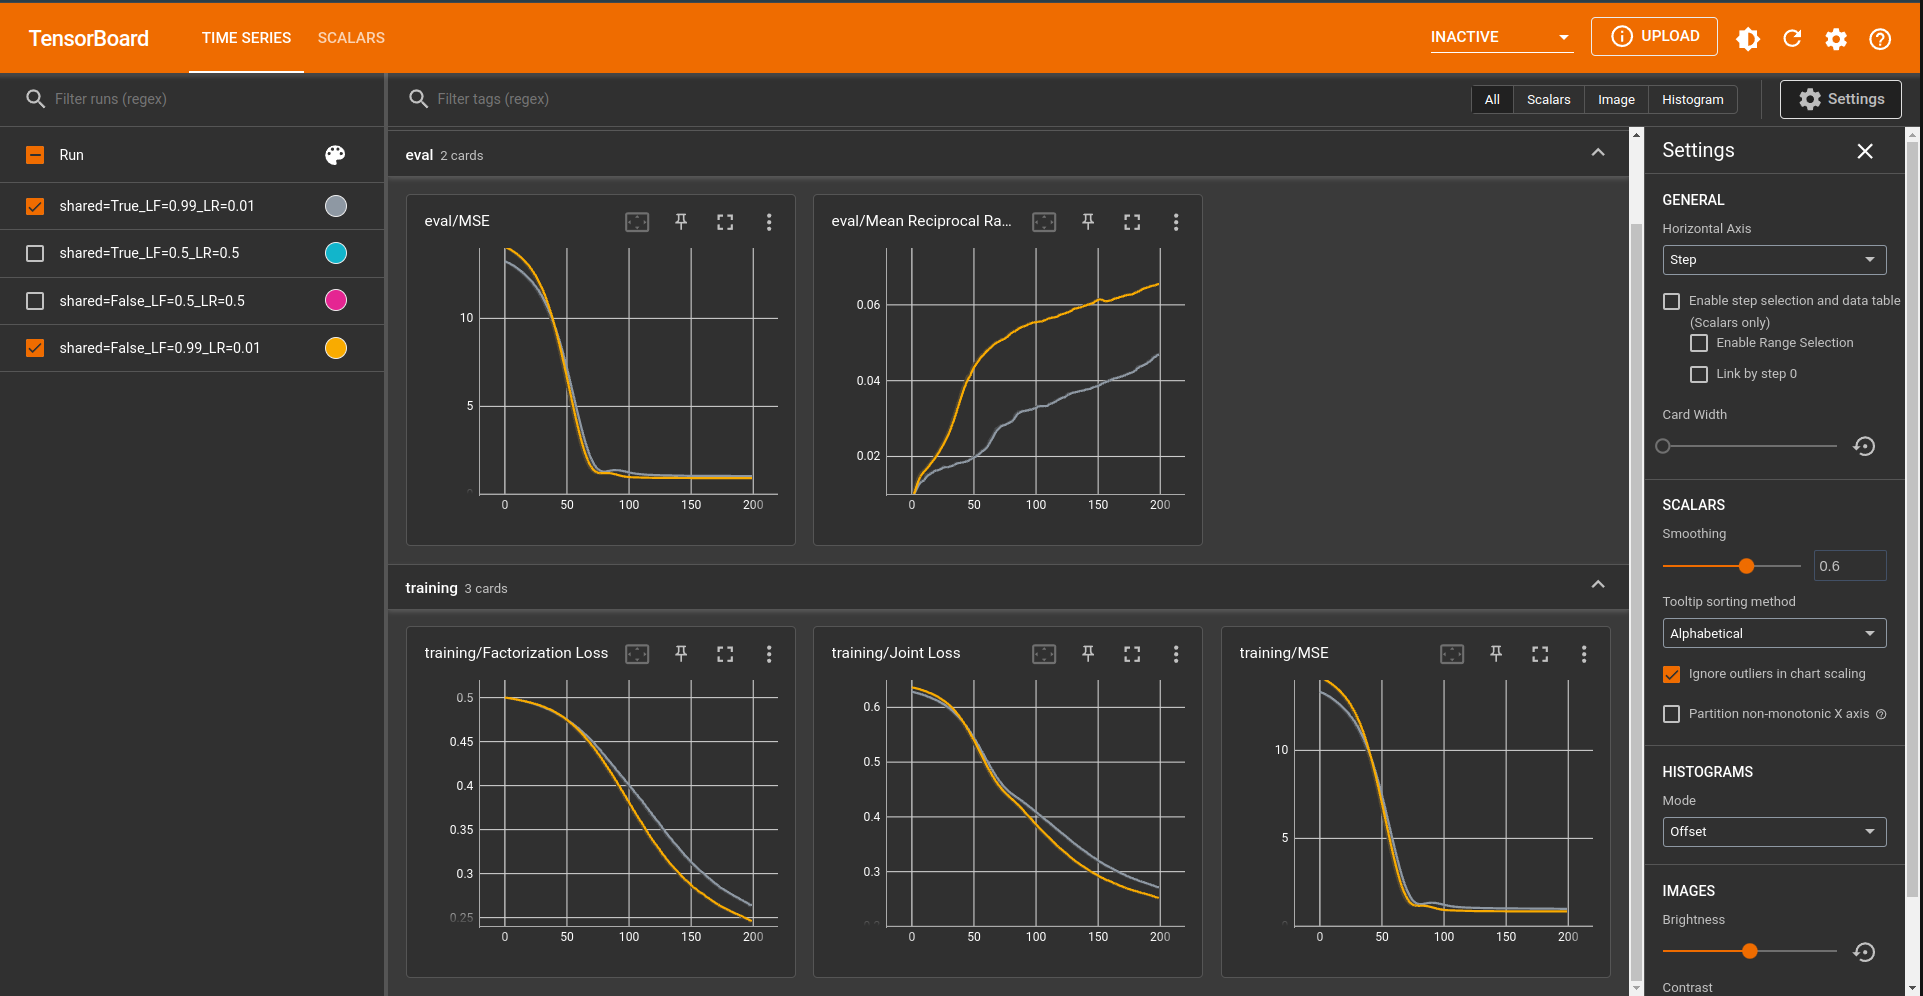
\includegraphics[width=1.0\textwidth]{LF99LR01}
	\end{center}
	Based on the train/test loss curves, parameter sharing does not outperform having separate models. \\
	Looking at the curves we see that the separate models model has a similar MSE for both eval and training implying that both parameter sharing and separate models performed equally on the regression task. \\
	The factorization and joint loss are lower and the Mean Reciprocal Rank is higher for the separate models model, impyling that the separate models model was more likely to recommend movies the user has seen than the shared parameters model.
    % ### END CODE HERE ###
\end{answer}
% <SCPD_SUBMISSION_TAG>_3a

\clearpage

\LARGE
3.b
\normalsize

% <SCPD_SUBMISSION_TAG>_3b
\begin{answer}
    % ### START CODE HERE ###
	\begin{center}
		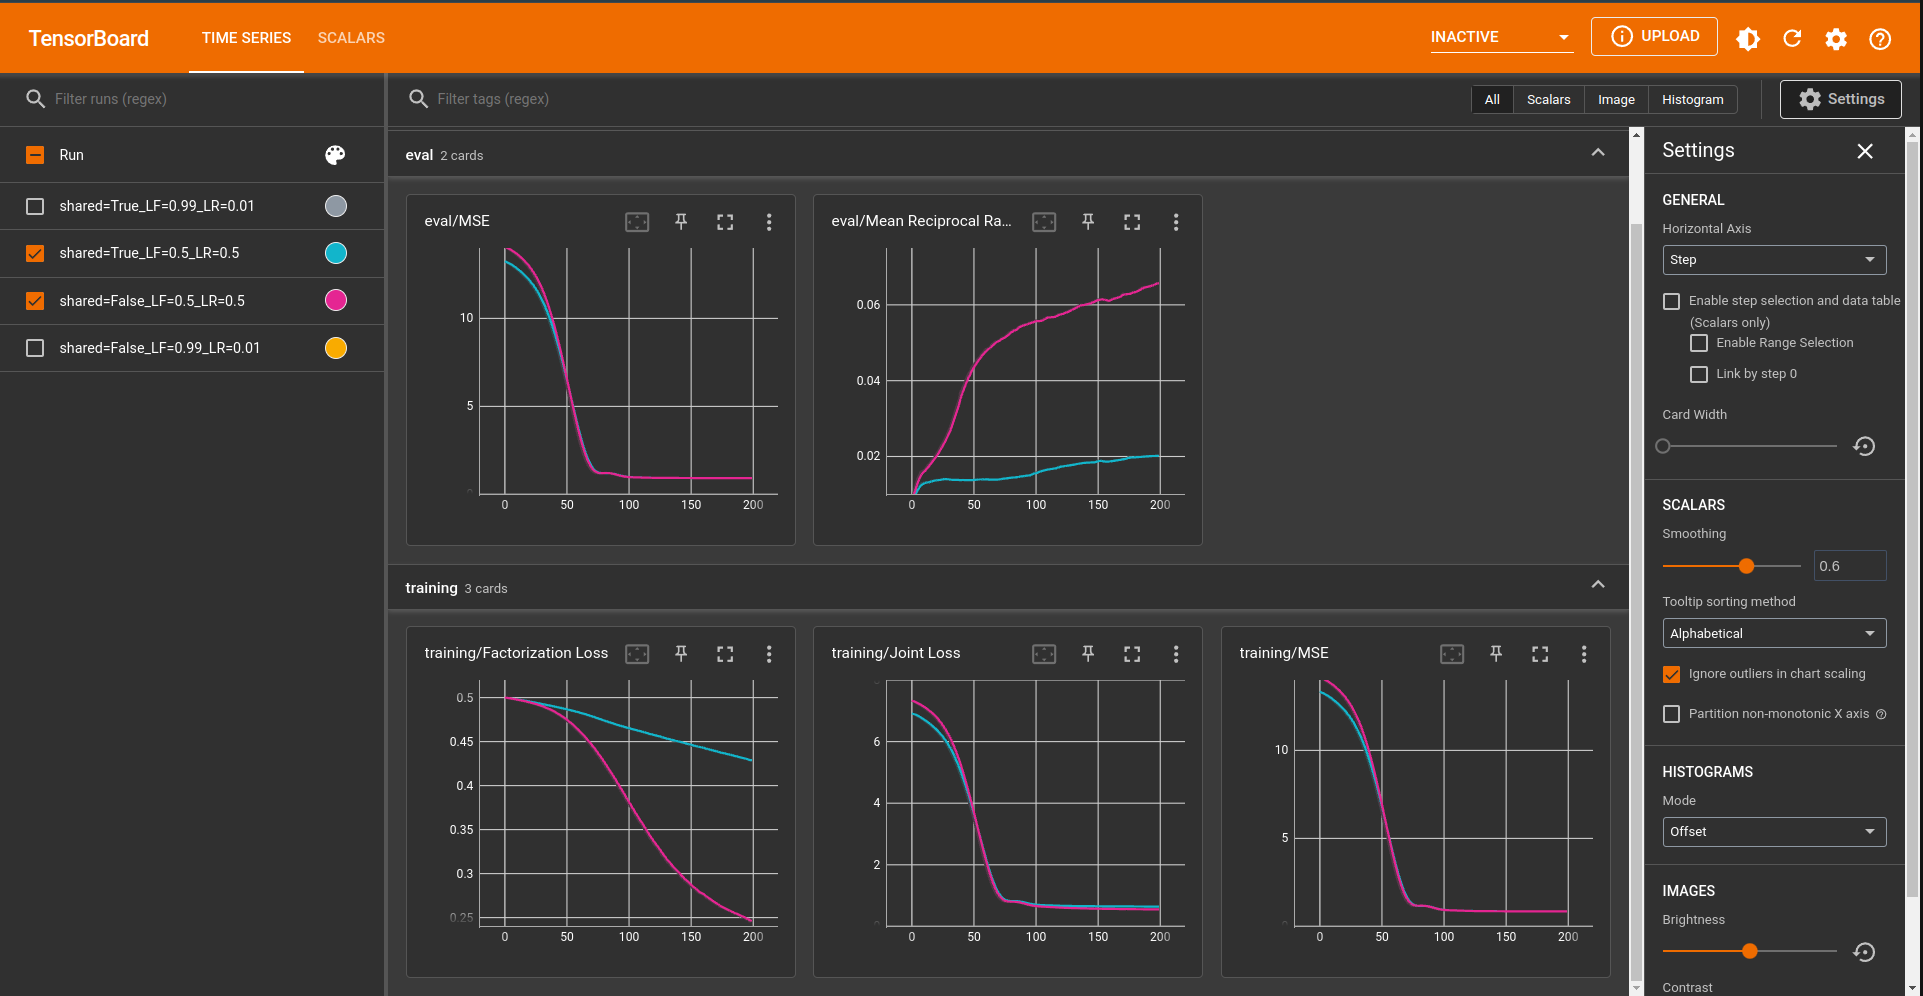
\includegraphics[width=1.0\textwidth]{LF05LR05}
	\end{center}
	Based on the train/test loss curves, parameter sharing does not outperform having separate models once again. \\
	First looking at the Joint Loss and MSE, parameter sharing and separate models look to produce similar results. \\
	However, when looking at Factorization loss we see that separate models is significantly lower. \\
	And when looking at the Mean Reciprical Rank we see once again that separate models is higher.
    % ### END CODE HERE ###
\end{answer}
% <SCPD_SUBMISSION_TAG>_3b

\clearpage

\LARGE
3.c
\normalsize

% <SCPD_SUBMISSION_TAG>_3c
\begin{answer}
    % ### START CODE HERE ###
	\begin{center}
		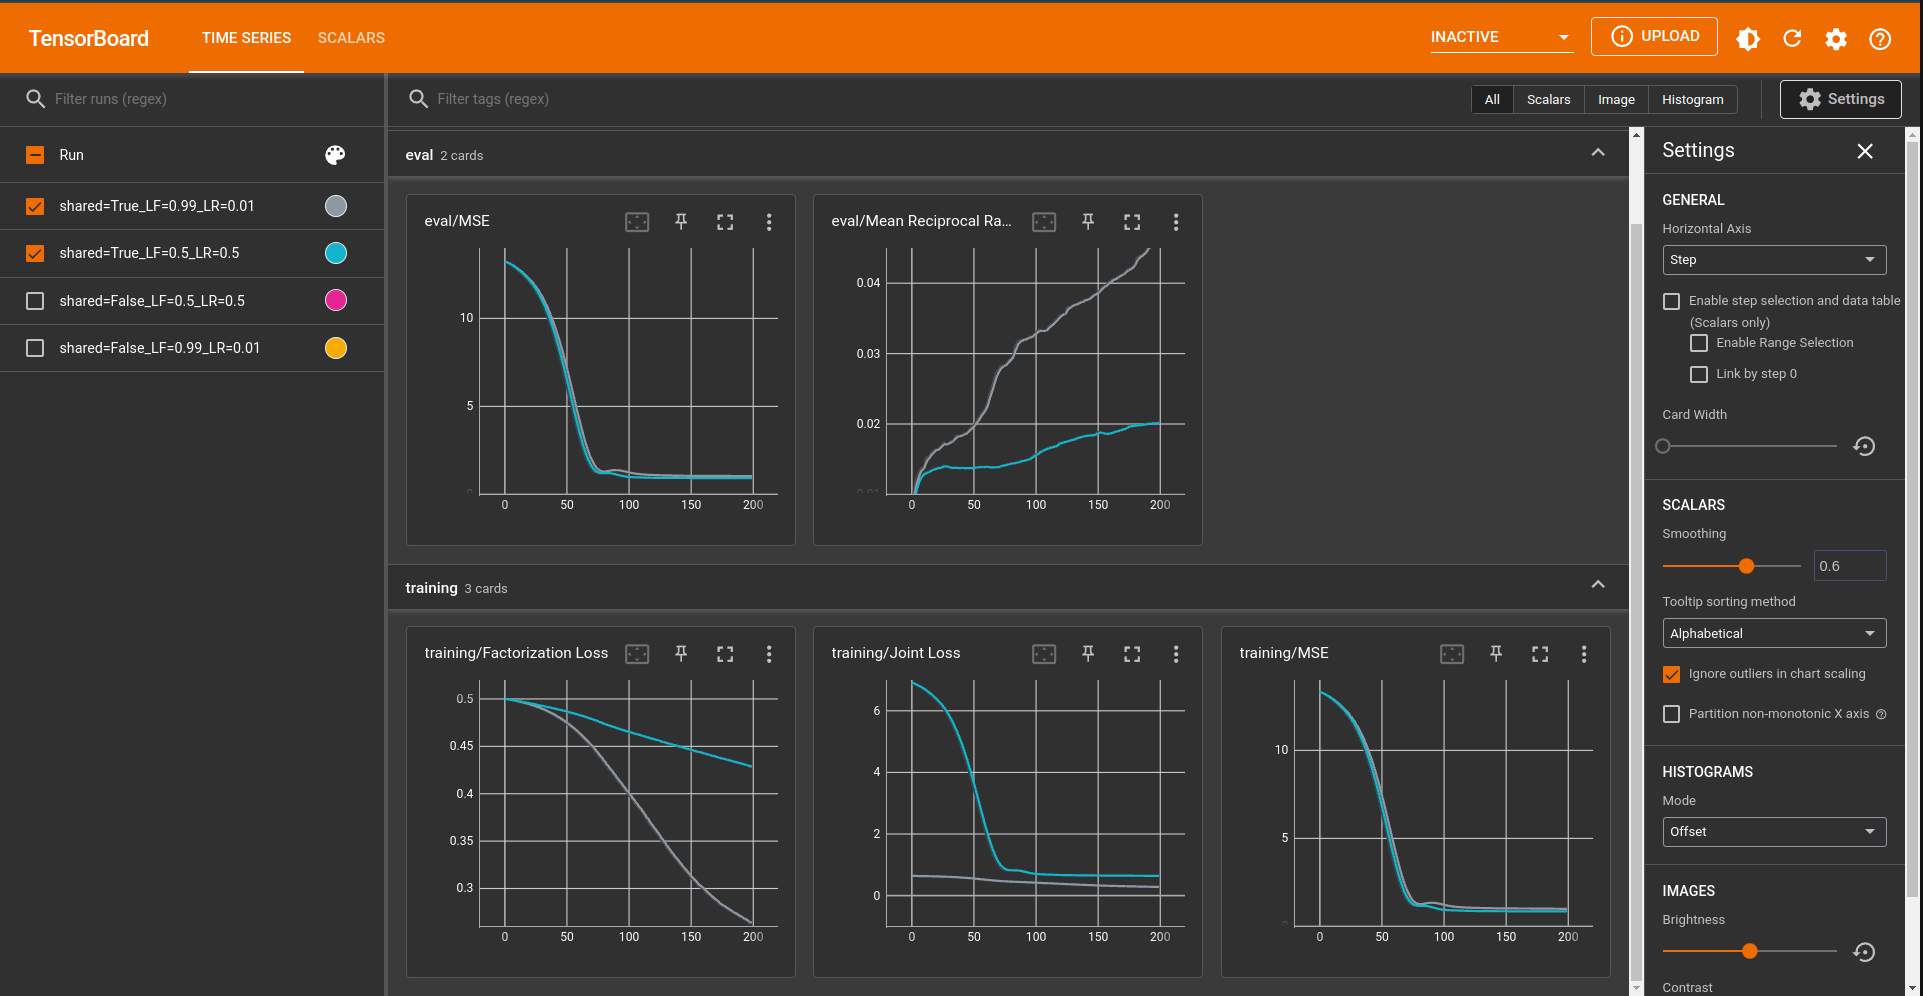
\includegraphics[width=1.0\textwidth]{SharedModelDifference}
	\end{center}
	Comparing the two shared models we see that they have similar performance on MSE loss. \\
	However, when comparing the Factorization and Joint Loss as well as the Mean Reciprocal Rank we see that the model with $\lambda_{F}$ = 0.99 $\lambda_{R} = 0.01$ converges faster. \\
	This performance difference makes sense as the model with $\lambda_{F}$ = 0.99 $\lambda_{R}$ = 0.01 is weighted in favor of the factorization task. \\
	Why does weighing the model in favor of the factorization task generate better results? \\
	I'm not entirely certain, but my best guess / intuition is that the factorization task is a more complicated task than the regression task and so the benefit of weighting in favor of the factorization task has a greater return than the performance drop in the regression task. This also seems like a good place to perform tuning to find the best "balance" between these parameters.
    % ### END CODE HERE ###
\end{answer}
% <SCPD_SUBMISSION_TAG>_3c

% <SCPD_SUBMISSION_TAG>_entire_submission

\end{document}
